\textcite{vlaanderen_staat_2019} estimated there were around 71.000 cases of Campylobacteriosis in the Netherlands in 2018, 67.000 in 2017 and 79.000 in 2016. We plotted the amount of cases produced by our model against the average of these three values. The results can be seen in Figure~\ref{fig:val_human_cases} Our model never exceeds that number, since it is a simplified version of reality, and certain disease vectors have been left out.

\textcite{nepluvi_rapportage_2019} monstered broiler chickens weekly in 2018, and found $41,9$-$58.1\%$ of broilerchickens were tested positive for \textit{Campylobacter}. This concerns chickens from slaughterhouses. As can be seen in Figure~\ref{fig:val_chickens}, in our model this number is an order of magnitude lower. NEED TO GIVE REASON

In the Netherlands the (unsanitary) preparation and / or consumption of chicken were attributed to $20$-$30\%$ of infections in 2018. However, around $50$-$80\%$ of cases can be attributed to \textit{Campylobacter} strains associated with poultry \parencite{cuperus_surveillance_2020, nepluvi_rapportage_2019}. Therefore, it is safe to assume that there are multiple transmission routes. We assume this transmission route can be found in the environment, and because of these facts, we assume the environmental transmission routes play a bigger role. Around $20$-$60\%$ of the human infections are from the environment. As can be seen in Figure~\ref{fig:val_sources} this is not the case in our model. The majority of the infections stem from food consumption. NEED TO GIVE REASON

We also validated our DALYs and Cost of Illness against the datapoints from RIVM. We plotted them against the average of the values mentioned in \citetitle{vlaanderen_staat_2019}. As can be seen in Figure~\ref{fig:val_dalys} our model determines higher DALYs than given in the literature. This indicates that in the real world there are a lot of cases of chronic diseases overlooked. There are probably a lot more chronic diseases that can be traced back to \textit{Campylobacter}. Perhaps the specialists are overlooking the bacterium as a cause, or they are simply unable to pinpoint the cause.

In Figure~\ref{fig:val_coi} it can be seen that the Cost of Illness calculated by the model is lower than the validation data. This is probably due to the fact that we only look at 3 chronic conditions and the acute conditions. It may also be the case \citeauthor{vlaanderen_staat_2019} has used a different value as the cost per condition. We based our indicators for the costs on the indicators used by \textcite{mangen_campylobacteriosis_2007}.

It is estimated there are around 17 million species of \textit{Diptera} per person \parencite{gorman_trillions_2017}. We are only interested in \textit{Musca domestica}. It is unknown what their numbers are in the Netherlands, and we are unable to estimate. However, it has been guessed that the population of Houseflies will increase by 244\% by 2080 \parencite{mcalister_secret_2017}. In The amount of flies in our model after 1 year is 20.000 of which 7.700 are infectious (TIME STEP = 0.0625). This is probably not a proper reflection of the real world, but one can assume that it is only 7.700 flies that have directly caused a disease in humans and/or chickens.

The model also includes an Infection risk from birds (2.5e-05). There are about 1.3 million birds in the Netherlands \parencite{noauthor_miljoenen_2019}. There was no literature on the risk from birds, so we assumed a somewhat safe value. We doubt \textit{Campylobacter} will ever be exterminated due to the presence of these environmental factors, even if we are somehow able to keep our farms, slaughterhouses and stores \textit{Campylobacter}free.

\begin{figure*}[!h]
    \centering
    \begin{minipage}{0.45\textwidth}
        \centering
        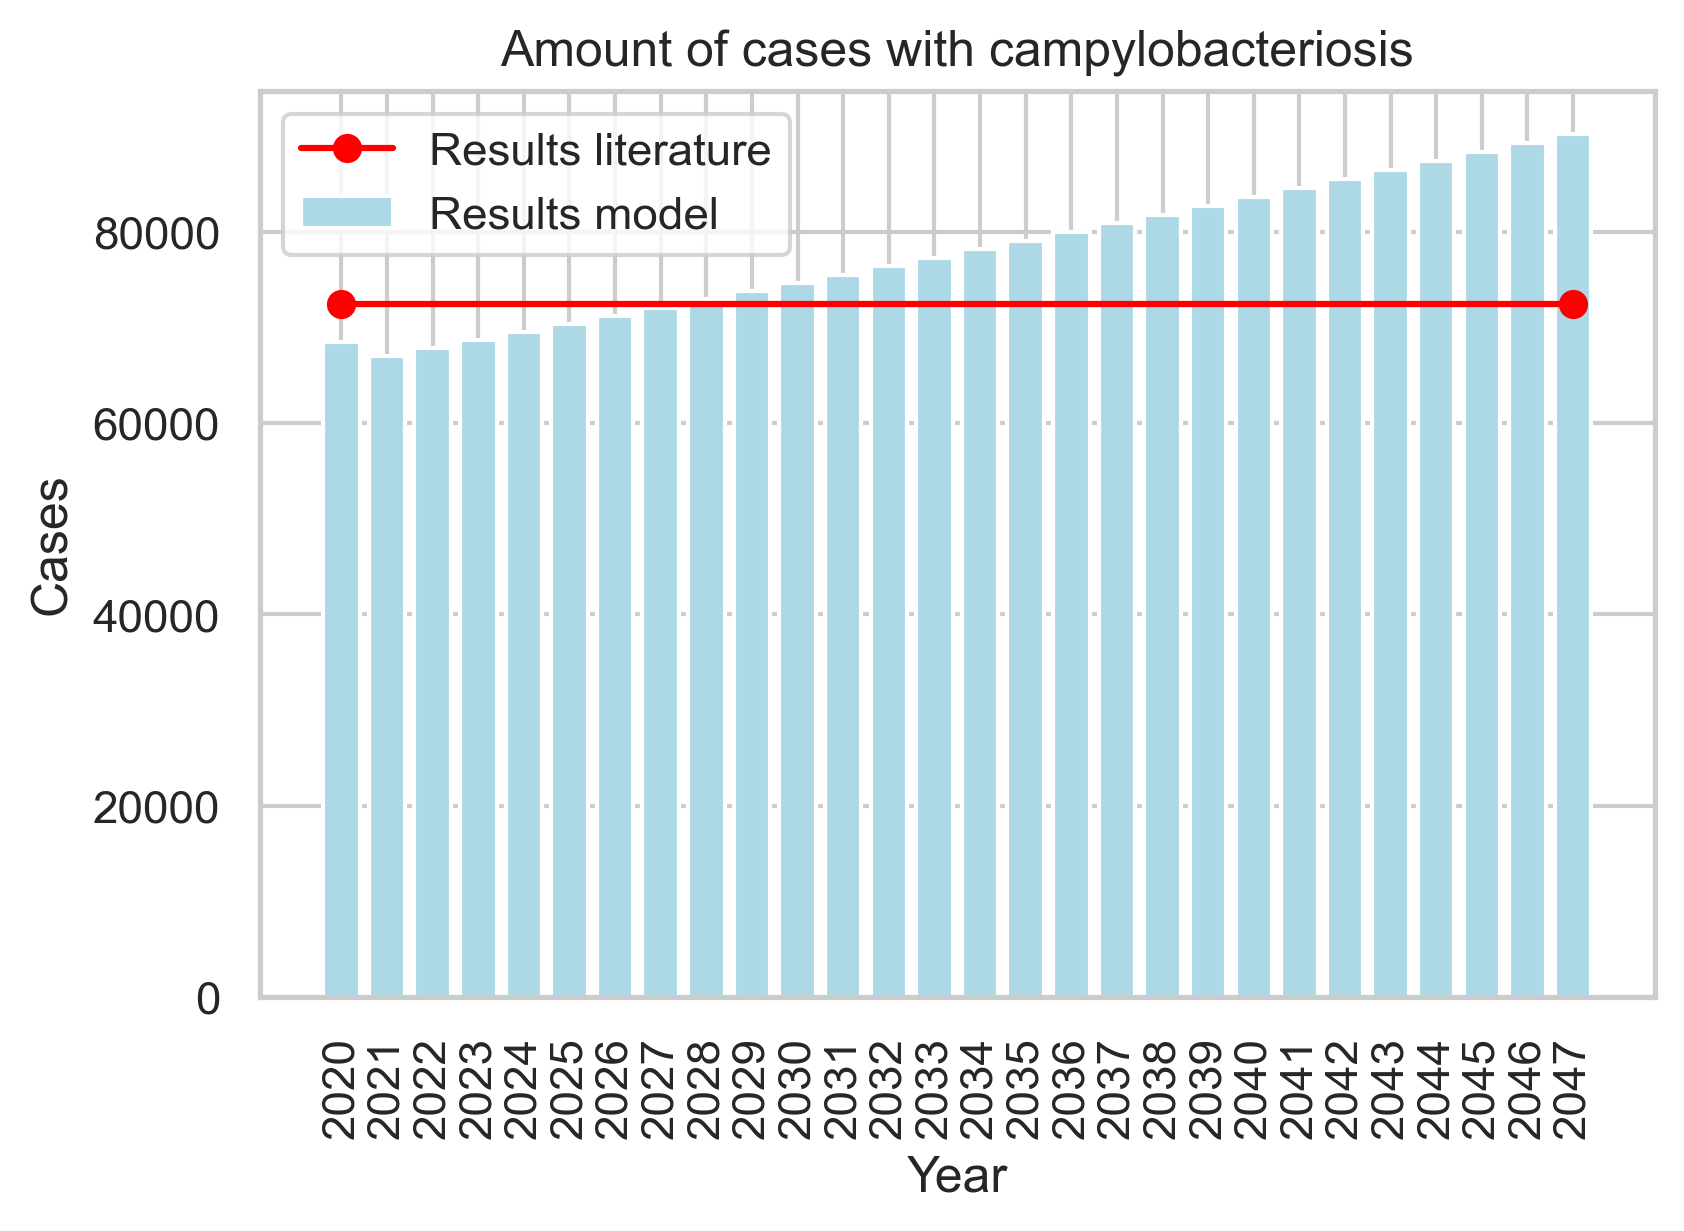
\includegraphics[width=0.9\textwidth]{notebooks/human_cases.png} % first figure itself
        \caption{Validation of human cases}
        \label{fig:val_human_cases}
    \end{minipage}\hfill
    \begin{minipage}{0.45\textwidth}
        \centering
        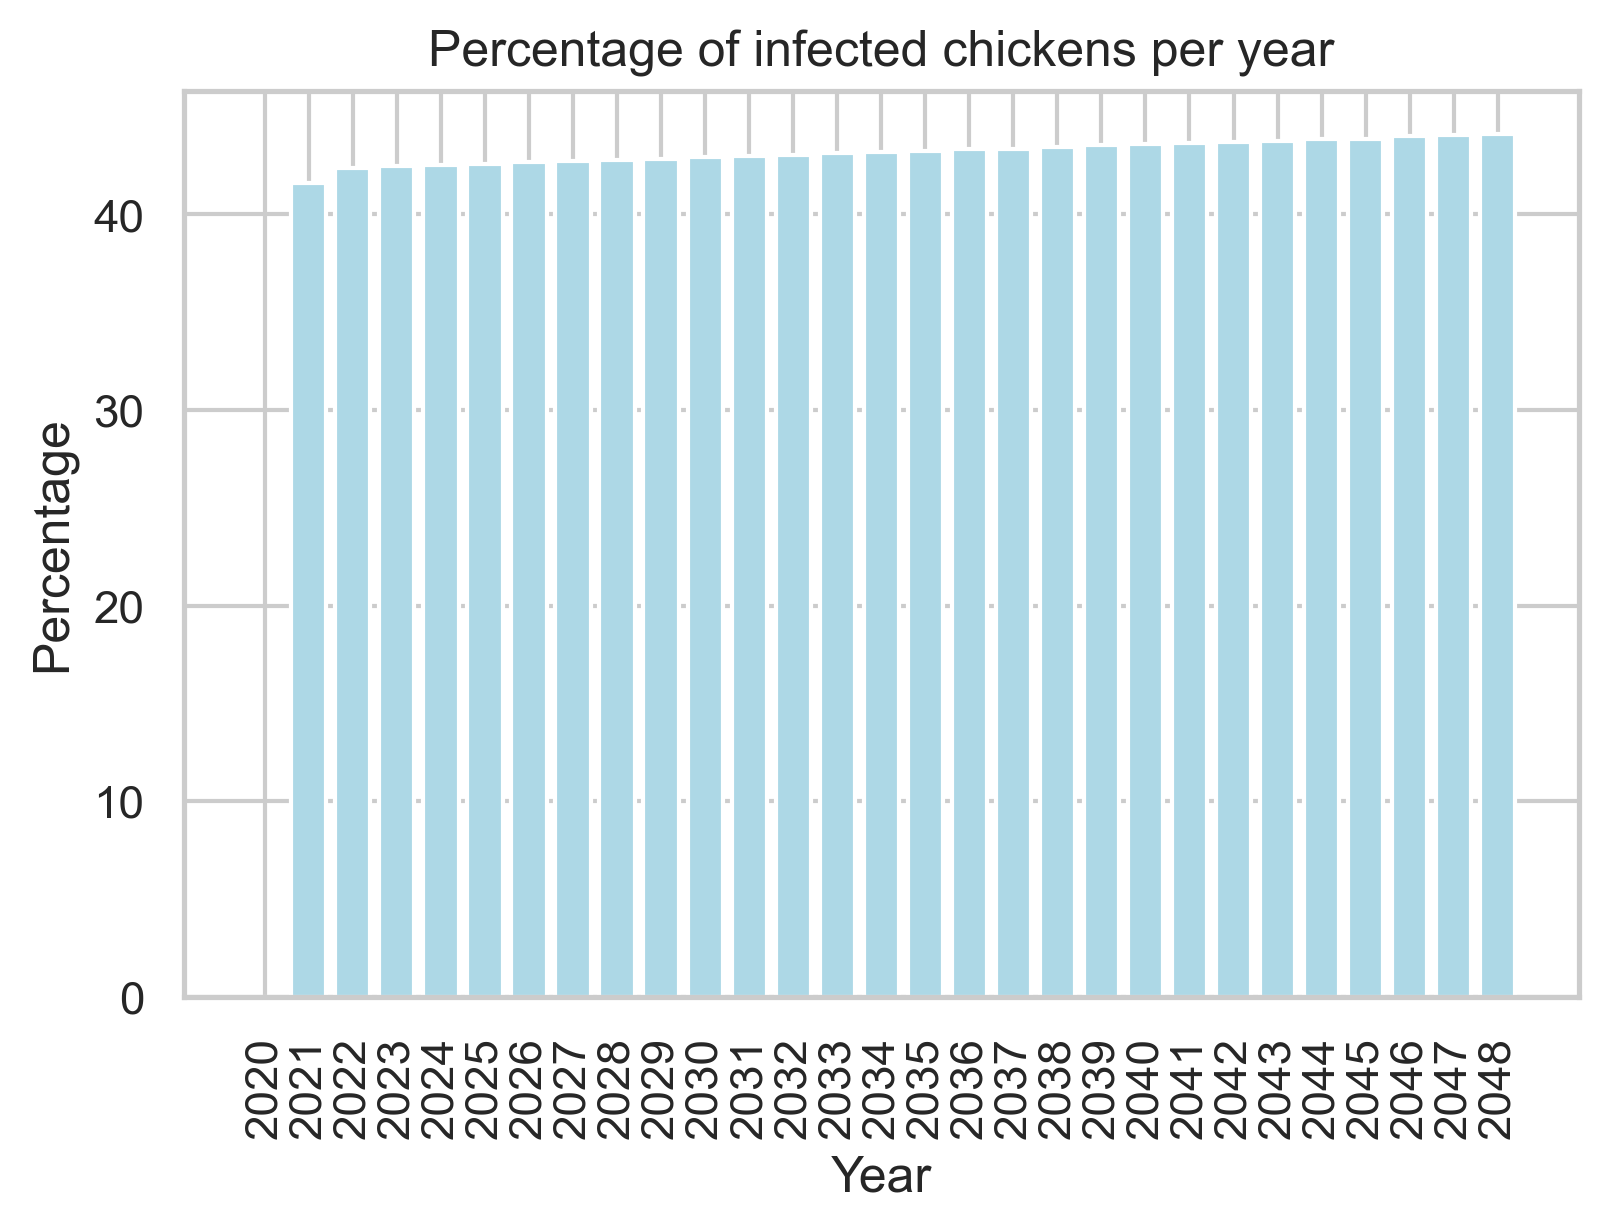
\includegraphics[width=0.9\textwidth]{notebooks/chickens.png} % second figure itself
        \caption{Validation of proportion infected chickens}
	    \label{fig:val_chickens}
    \end{minipage}
\end{figure*}

\begin{figure*}[!h]
	\centering
	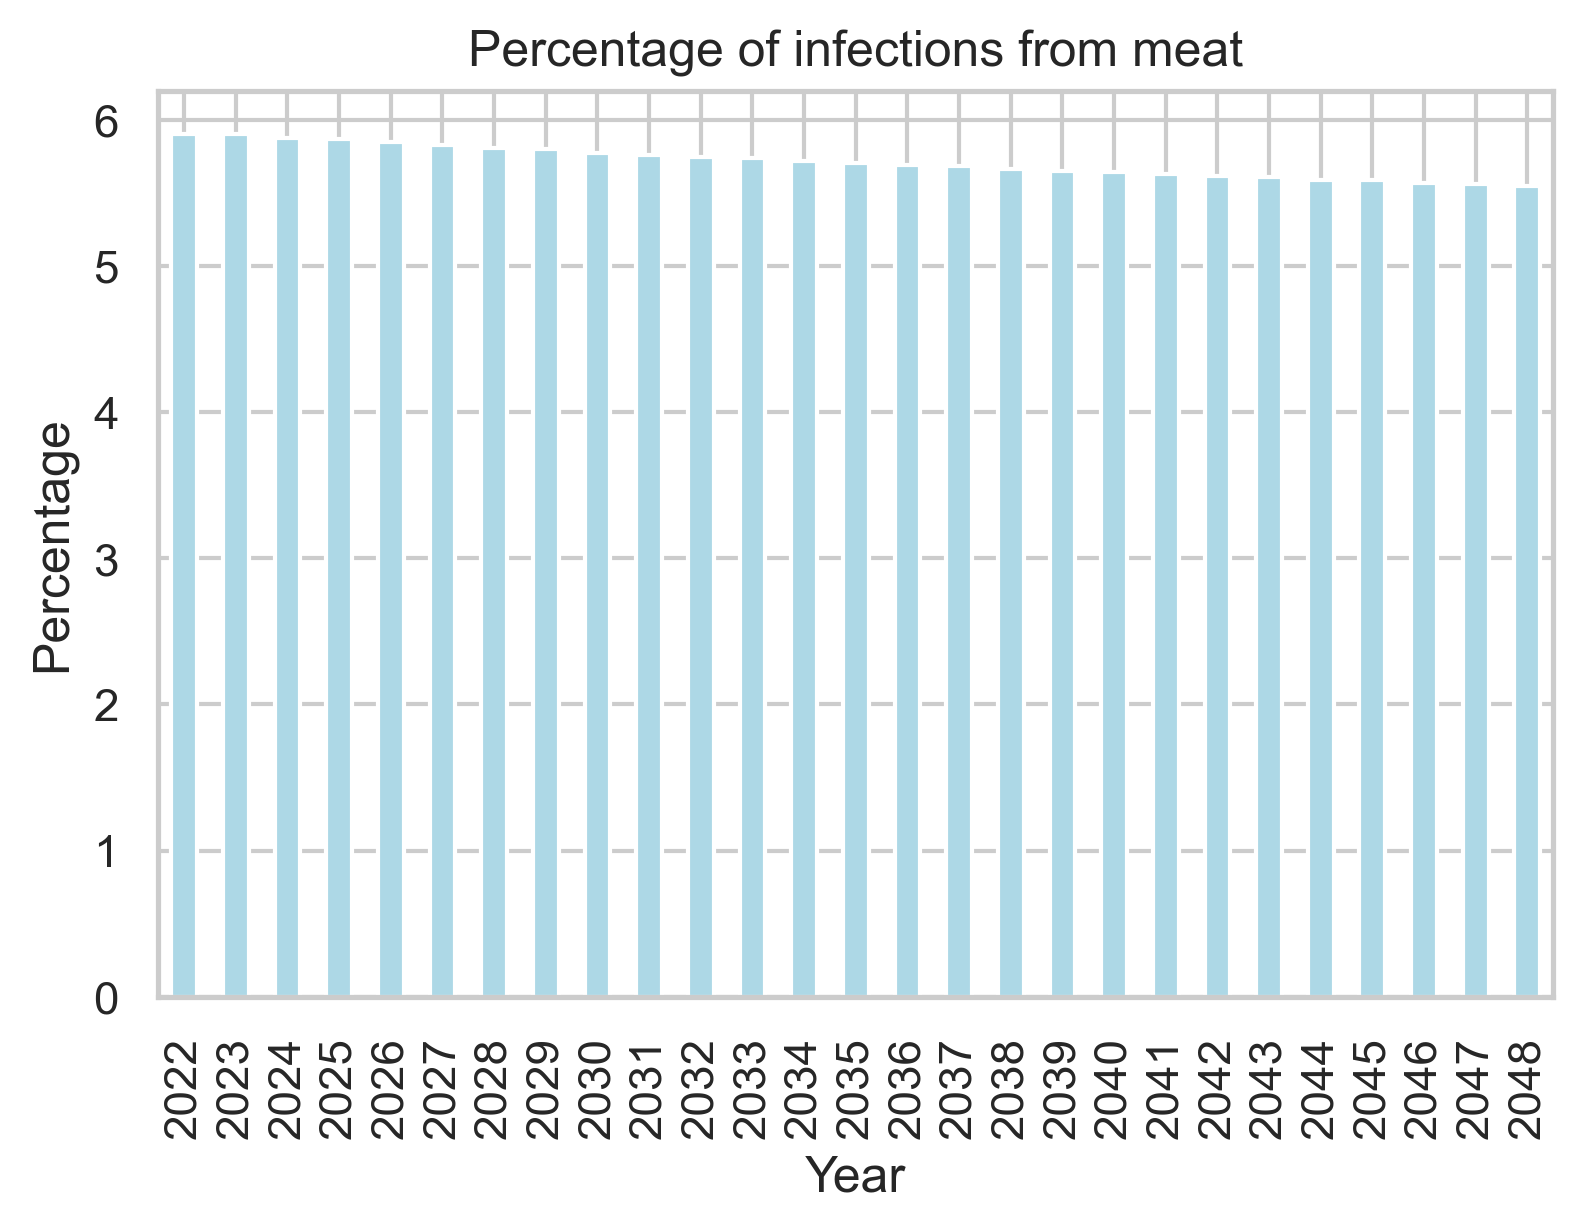
\includegraphics[width=0.5\textwidth]{notebooks/source.png}
	\caption{Validation of sources of Campylobacteriosis}
	\label{fig:val_sources}
\end{figure*}

\begin{figure*}[!h]
    \centering
    \begin{minipage}{0.45\textwidth}
        \centering
        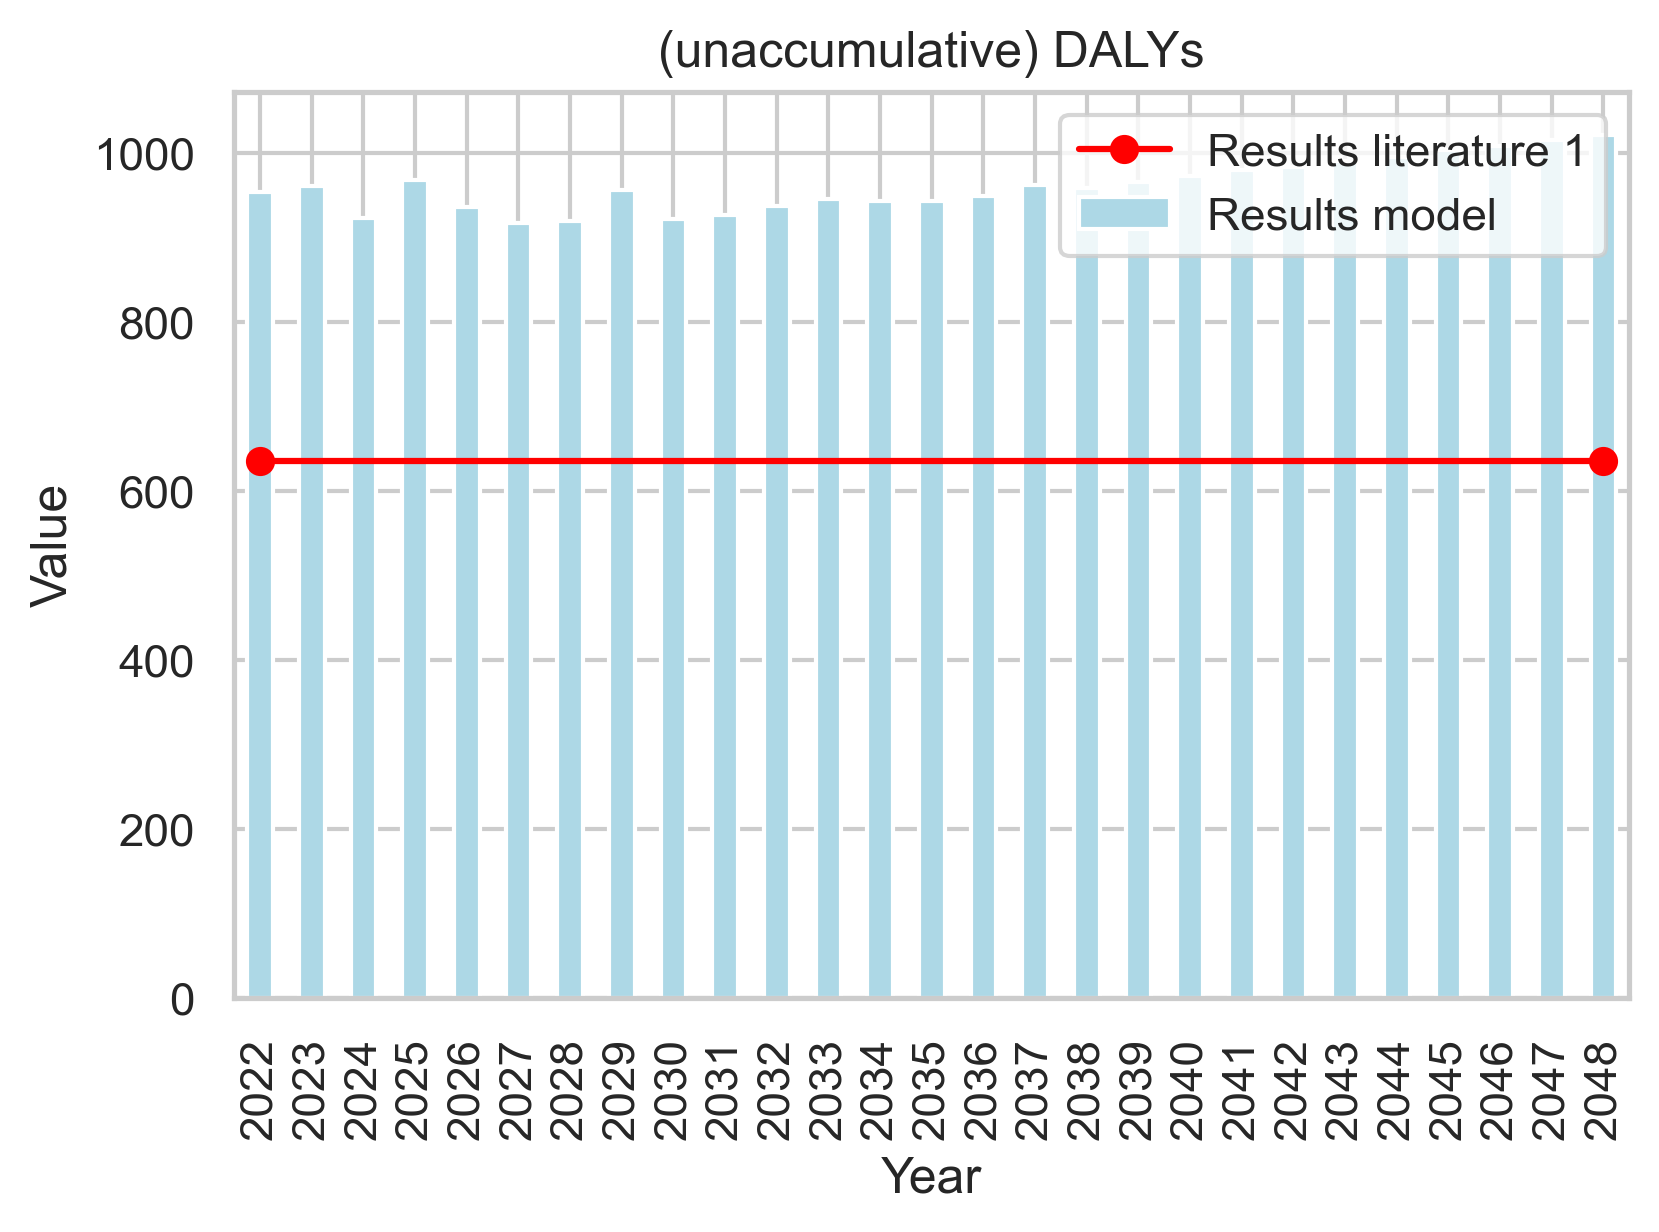
\includegraphics[width=0.9\textwidth]{notebooks/dalys.png} % first figure itself
        \caption{Validation of DALYs}
	    \label{fig:val_dalys}
    \end{minipage}\hfill
    \begin{minipage}{0.45\textwidth}
        \centering
        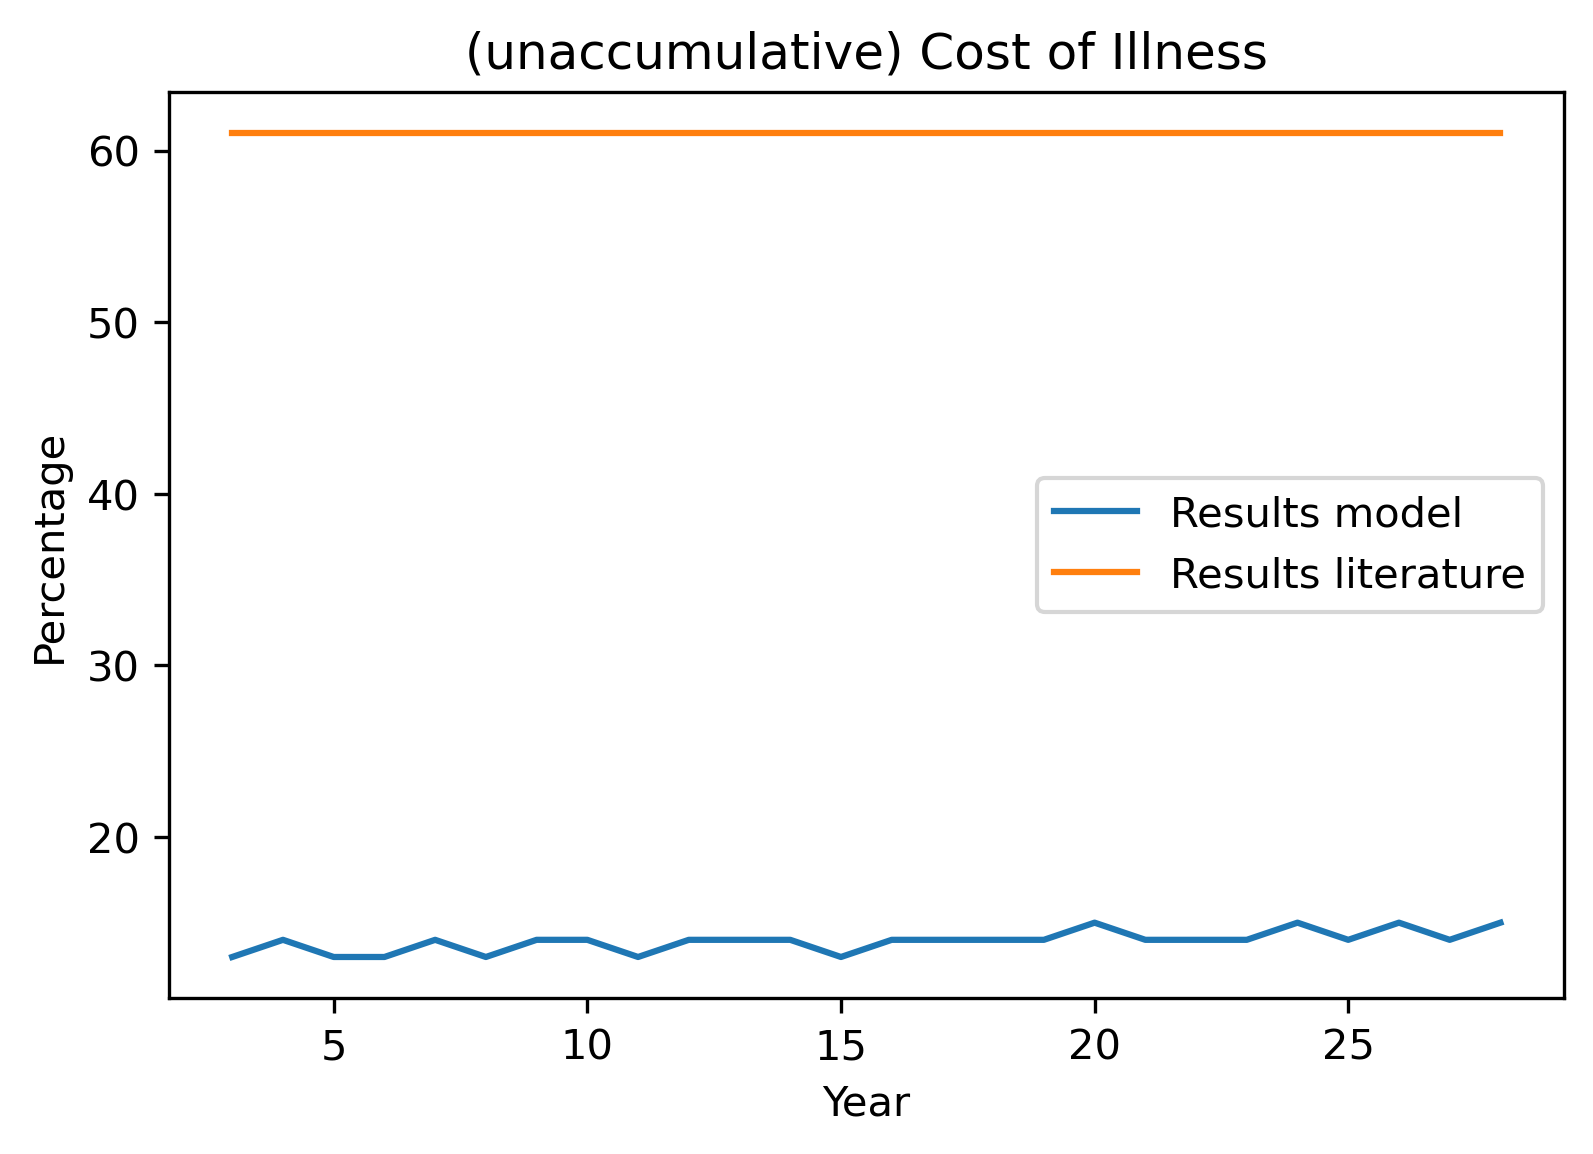
\includegraphics[width=0.9\textwidth]{notebooks/coi.png} % second figure itself
        \caption{Validation of Cost of Illness}
	    \label{fig:val_coi}
    \end{minipage}
\end{figure*}